\documentclass[letterpaper]{article}\usepackage[]{graphicx}\usepackage[]{color}
%% maxwidth is the original width if it is less than linewidth
%% otherwise use linewidth (to make sure the graphics do not exceed the margin)
\makeatletter
\def\maxwidth{ %
  \ifdim\Gin@nat@width>\linewidth
    \linewidth
  \else
    \Gin@nat@width
  \fi
}
\makeatother

\definecolor{fgcolor}{rgb}{0, 0, 0}
\newcommand{\hlnum}[1]{\textcolor[rgb]{0.502,0,0.502}{\textbf{#1}}}%
\newcommand{\hlstr}[1]{\textcolor[rgb]{0.651,0.522,0}{#1}}%
\newcommand{\hlcom}[1]{\textcolor[rgb]{1,0.502,0}{#1}}%
\newcommand{\hlopt}[1]{\textcolor[rgb]{1,0,0.502}{\textbf{#1}}}%
\newcommand{\hlstd}[1]{\textcolor[rgb]{0,0,0}{#1}}%
\newcommand{\hlkwa}[1]{\textcolor[rgb]{0.733,0.475,0.467}{\textbf{#1}}}%
\newcommand{\hlkwb}[1]{\textcolor[rgb]{0.502,0.502,0.753}{\textbf{#1}}}%
\newcommand{\hlkwc}[1]{\textcolor[rgb]{0,0.502,0.753}{#1}}%
\newcommand{\hlkwd}[1]{\textcolor[rgb]{0,0.267,0.4}{#1}}%

\usepackage{framed}
\makeatletter
\newenvironment{kframe}{%
 \def\at@end@of@kframe{}%
 \ifinner\ifhmode%
  \def\at@end@of@kframe{\end{minipage}}%
  \begin{minipage}{\columnwidth}%
 \fi\fi%
 \def\FrameCommand##1{\hskip\@totalleftmargin \hskip-\fboxsep
 \colorbox{shadecolor}{##1}\hskip-\fboxsep
     % There is no \\@totalrightmargin, so:
     \hskip-\linewidth \hskip-\@totalleftmargin \hskip\columnwidth}%
 \MakeFramed {\advance\hsize-\width
   \@totalleftmargin\z@ \linewidth\hsize
   \@setminipage}}%
 {\par\unskip\endMakeFramed%
 \at@end@of@kframe}
\makeatother

\definecolor{shadecolor}{rgb}{.97, .97, .97}
\definecolor{messagecolor}{rgb}{0, 0, 0}
\definecolor{warningcolor}{rgb}{1, 0, 1}
\definecolor{errorcolor}{rgb}{1, 0, 0}
\newenvironment{knitrout}{}{} % an empty environment to be redefined in TeX

\usepackage{alltt}
%\VignetteIndexEntry{Algorightms and Equations}
%\VignetteEngine{knitr::knitr}
\usepackage{graphicx}
\usepackage[colorlinks = true,
            urlcolor = blue,
            citecolor = blue,
            linkcolor = blue]{hyperref}
\usepackage{array}
\usepackage{color}
\usepackage[usenames,dvipsnames,svgnames,table]{xcolor}
\usepackage[utf8]{inputenc} % for UTF-8/single quotes from sQuote()
\usepackage{fullpage}
\usepackage{mathtools}
\usepackage{makeidx}
\usepackage{longtable}

% for bold symbols in mathmode
\usepackage{bm}
\newcommand{\R}{\mathbb{R}}
\newcommand{\m}[1]{\mathbf{#1}}
\newcommand{\tab}{\hspace*{1em}}
\newcolumntype{H}{>{\setbox0=\hbox\bgroup}c<{\egroup}@{}}
\newcommand{\cmdlink}[2]{%
  \texttt{\hyperref[#1]{#2}}%
}
\newcommand{\seclink}[2]{%
  \textsc{\hyperref[#1]{#2}}%
}

\newcommand{\poppr}{\textit{poppr}}
\newcommand{\Poppr}{\textit{Poppr}}
\newcommand{\adegenet}{\textit{adegenet}}
\newcommand{\Adegenet}{\textit{Adegenet}}
\newcommand{\tline}{
  \noindent
  \rule{\textwidth}{1pt}
  \par
}
\newcommand{\bline}{
  \noindent
  \rule{\textwidth}{1pt}
  \kern1pt
}

\newcommand{\jala}{
  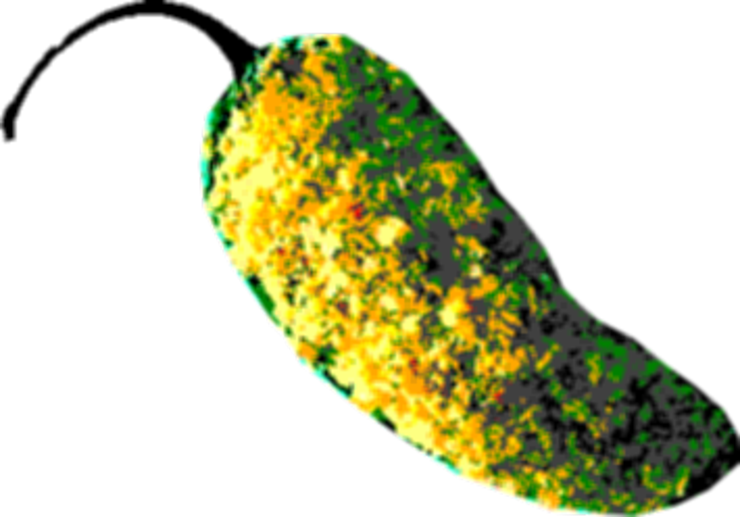
\includegraphics[height = 5mm, keepaspectratio=true]{jalapeno-poppers}
}

\newcommand{\revjala}{
  \scalebox{-1}[1]{\jala{}}
}

\title{Algorithms and equations utilized in poppr version 1.1.0}
\author{Zhian N. Kamvar$^{1}$\ and Niklaus J. Gr\"unwald$^{1,2}$\\\scriptsize{1)
Department of Botany and Plant Pathology, Oregon State University, Corvallis,
OR}\\\scriptsize{2) Horticultural Crops Research Laboratory, USDA-ARS,
Corvallis, OR}}
\IfFileExists{upquote.sty}{\usepackage{upquote}}{}
\begin{document}


\maketitle

\begin{abstract}
This vignette is focused on simply explaining the different algorithms utilized
in calculations such as the index of association and different distance measures.
Many of these are previously described in other papers and it would be prudent
to cite them properly if they are used.
\end{abstract}

% \begin{figure}[b]   
%   \centering
%   \label{logo}   
%   
\includegraphics{popprlogo} 
% \end{figure} 
% 
% \newpage 
\begingroup
  \hypersetup{linkcolor=black} 
  \tableofcontents 
\endgroup 

\section{Mathematical representation of data in \adegenet{} and \poppr{}}

The sections dealing with the index of association and genetic distances will be
based on the same data structure, a matrix with samples in rows and alleles in
columns. The number of columns is equal to the total number of alleles observed
in the data set. Much of this description is derived from \adegenet{}'s
\texttt{dist.genpop} manual page.

\begin{quote}
Let \textbf{A} be a table containing allelic frequencies with $t$
samples\footnote{populations or individuals} (rows) and $m$ alleles (columns).\\
\end{quote}
The above statement describes the table present in genind or genpop object
where, instead of having the number of columns equal the number of loci, the
number of columns equals the number of observed alleles in the entire data set.

\begin{quote}
Let $\nu$ be the number of loci. The locus $j$ gets $m(j)$ alleles. 

\begin{equation}
  m=\sum_{j=1}^{\nu} m(j)
\end{equation}
\end{quote}

So, if you had a data set with 5 loci that had 2 alleles each, your table
would have ten columns. Of course, codominant loci like microsatellites have
varying numbers of alleles.


\begin{quote}
For the row $i$ and the modality $k$ of the variable $j$, notice the value

\begin{equation}
  a_{ijk}\\ (1 \leq i \leq t,\\ 1 \leq j \leq \nu,\\ 1 \leq k \leq m(j))
\end{equation}

\begin{equation}
  a_{ij\cdot}=\sum_{k=1}^{m(j)}a_{ijk} 
\end{equation}

\begin{equation}
  p_{ijk}=\frac{a_{ijk}}{a_{ij\cdot}}
\end{equation}
\end{quote}

The above couple of equations are basically defining the allele counts
($a_{ijk}$) and frequency ($p_{ijk}$). Remember that $i$ is individual, $j$ is
locus, and $k$ is allele. The following continues to describe properties of the
frequency table used for analysis:

\begin{quote}
\begin{equation}
 p_{ij\cdot}=\sum_{k=1}^{m(j)}p_{ijk}=1
\end{equation}
\end{quote}
The sum of all allele frequencies for a single population (or individual) at a 
single locus is one.

\begin{quote}
\begin{equation}
p_{i{\cdot}\cdot}=\sum_{j=1}^{\nu}p_{ij\cdot}=\nu
\end{equation}
\end{quote}
The sum of all allele frequencies over all loci is equal to the number of loci.

\begin{quote} 
\begin{equation}
p_{{\cdot}{\cdot}\cdot}=\sum_{j=1}^{\nu}p_{i{\cdot}\cdot}=t\nu
\end{equation}
\end{quote}
The the sum of the entire table is the sum of all loci multiplied by the number 
of populations (or individuals).


% %
% %-----------------------------------------------------------------------------%
% %


\section{The Index of Association}
\label{indexassoc}

The index of association was originally developed by A.H.D. Brown analyzing
population structure of wheat and has been widely used as a tool to detect
clonal reproduction within populations \cite{Brown:1980, Smith:1993}.
Populations whose members are undergoing sexual reproduction, whether it be
selfing or out-crossing, will produce gametes via meiosis, and thus have a
chance to shuffle alleles in the next generation. Populations whose members are
undergoing clonal reproduction, however, generally do so via mitosis.

The most likely mechanism, therefor for a change in genotype for a clonal organism is via
mutation. The rate of mutation varies from species to species, but it is rarely
sufficiently high to approximate a random shuffling of alleles. The index of
association is a calculation based on the ratio of the variance of the raw
number of differences between individuals and the sum of those variances over
each locus \cite{Smith:1993}. It can also be thought of as the observed variance
over the expected variance. If both variances are equal, then the index is zero
after subtracting one (from Maynard-Smith, 1993 \cite{Smith:1993}):
\begin{equation}
\label{eq:I_A}
I_A = \frac{V_O}{V_E}-1
\end{equation}
Any sort of marker can be used for this analysis as it only counts differences
between pairs of samples. This can be thought of as a distance whose maximum is
equal to the number of loci multiplied by the ploidy of the sample. This is
calculated using an absolute genetic distance.

Remember that in \poppr{}, genetic data is stored in a table where the rows
represent samples and the columns represent potential allelic states grouped by
locus. Notice also that the sum of the rows all equal one. \Poppr{} uses this to
calculate distances by simply taking the sum of the absolute values of the
differences between rows.

The calculation for the distance between two individuals at a single locus $j$
with $m(j)$ allelic states and a ploidy of $l$ is as follows\footnote{Individuals
with Presence / Absence data will have the $l/2$ term dropped.}:
\begin{equation}
\label{eq:ia_d}
  d(a,b)=\frac{l}{2} \sum_{k=1}^{m(j)}
  |p_{ajk} - p_{bjk}|
\end{equation}

% \begin{equation}

% d = \displaystyle \frac{k}{2}\sum_{i=1}^{a} \mid ind_{Ai} - ind_{Bi}\mid
% \end{equation}
\noindent
To find the total number of differences between two individuals over all loci,
you just take $d$ over $\nu$ loci, a value we'll call $D$:

\begin{equation}
\label{eq:ia_D}
D(a,b) = \displaystyle \sum_{i=1}^{\nu} d_i
\end{equation}
An interesting observation: $D(a,b)/(l\nu)$ is Provesti's distance.

These values are calculated over all possible combinations of individuals in the
data set, ${n \choose 2}$ after which you end up with ${n \choose 2}\cdot{}\nu$
values of $d$ and ${n \choose 2}$ values of $D$. Calculating the observed
variances is fairly straightforward (modified from Agapow and Burt, 2001)
\cite{Agapow:2001}:

\begin{equation}
\label{eq:V_O}
V_O = \frac{\displaystyle \sum_{i=1}^{n \choose 2} D_{i}^2 - \frac{\left(\displaystyle\sum_{i=1}^{n \choose 2} D_{i}\right)^2}{{n \choose 2}}}{{n \choose 2}}
\end{equation}

Calculating the expected variance is the sum of each of the variances of the
individual loci. The calculation at a single locus, $j$ is the same as the
previous equation, substituting values of $D$ for $d$ \cite{Agapow:2001}:

\begin{equation}
\label{eq:var_j}
var_j = \frac{\displaystyle \sum_{i=1}^{n \choose 2} d_{i}^2 - \frac{\left(\displaystyle\sum_{i=1}^{n \choose 2} d_i\right)^2}{{n \choose 2}}}{{n \choose 2}}
\end{equation}

The expected variance is then the sum of all the variances over all $\nu$ loci
\cite{Agapow:2001}:

\begin{equation}
\label{eq:V_E}
V_E = \displaystyle \sum_{j=1}^{\nu} var_j
\end{equation}

Now you can plug the sums of equations (\ref{eq:V_O}) and (\ref{eq:V_E}) into
equation (\ref{eq:I_A}) to get the index of association. Of course, Agapow and
Burt showed that this index increases steadily with the number of loci, so they
came up with an approximation that is widely used, $\bar r_d$
\cite{Agapow:2001}. For the derivation, see the manual for \textit{multilocus}.
The equation is as follows, utilizing equations (\ref{eq:V_O}),
(\ref{eq:var_j}), and (\ref{eq:V_E}) \cite{Agapow:2001}:

\begin{equation}
\label{eq:r_d}
\bar{r}_d = \frac{V_O - V_E}
{2\displaystyle \sum_{j=1}^{\nu}\displaystyle \sum_{k \neq j}^{\nu}\sqrt{var_j\cdot{}var_k}}
\end{equation}

\section{Genetic distances}

Genetic distances are great tools for analyzing diversity in
populations as they are the basis for creating dendrograms with bootstrap
support and also for AMOVA. This section will simply present different genetic
distances along with a few notes about them. Most of these distances are derived
from the \textit{ade4} and \adegenet{} packages, where they were implemented as
distances between populations. \Poppr{} extends the implementation to individuals
as well (with the exception of Bruvo's distance).

\begin{table}[ht]
\centering
\caption{Distance measures and their respective assumptions}
\begin{tabular}{lllll}
  \hline
 Method & Function & Assumption & Euclidean & Citation\\ 
  \hline
Provesti & \texttt{provesti.dist} & - & No & \cite{prevosti1975distances}\\
 & \texttt{diss.dist} & & & \\
Nei & \texttt{nei.dist} & Infinite Alleles & No & \cite{nei1972genetic, nei1978estimation}\\
 & & Genetic Drift & & \\
Edwards & \texttt{edwards.dist} & Genetic Drift & Yes & \cite{edwards1971distances}\\
Reynolds & \texttt{reynolds.dist} & Genetic Drift & Yes & \cite{reynolds1983estimation}\\
Rogers & \texttt{rogers.dist} & - & Yes & \cite{rogers1972measures}\\
Bruvo & \texttt{bruvo.dist} & Stepwise Mutation & No & \cite{Bruvo:2004}\\
   \hline
\end{tabular}
\end{table}

\subsection{Distances that assume genetic drift}
\subsubsection{Nei's 1978 Distance}
\label{distance:nei}
\begin{equation}
  D_{Nei}(a,b)= -\ln\left(\frac{\sum_{k=1}^{\nu} \sum_{j=1}^{m(k)}
  p_{ajk} p_{bjk}}{\sqrt{\sum_{k=1}^{\nu} \sum_{j=1}^{m(k)}
  {(p_{ajk}) }^2}\sqrt{\sum_{k=1}^{\nu} \sum_{j=1}^{m(k)}
  {(p_{bjk})}^2}}\right)
\end{equation}

Note: if comparing individuals in \poppr{}, those that do not share any alleles
normally receive a distance of $\infty$. As you cannot draw a dendrogram with 
infinite branch lengths, these are converted to an order of magnitude higher
distance than the largest observed less than $\infty$.

\subsubsection{Edwards' angular distance}
\label{distance:edwards}
\begin{equation}
  D_{Edwards}(a,b)=\sqrt{1-\frac{1}{\nu} \sum_{k=1}^{\nu}
  \sum_{j=1}^{m(k)} \sqrt{p_{ajk}  p_{bjk}}}
\end{equation}

\subsubsection{Reynolds' coancestry distance}
\label{distance:reynolds}
\begin{equation}
  D_{Reynolds}(a,b)=\sqrt{\frac{\sum_{k=1}^{\nu}
  \sum_{j=1}^{m(k)}{(p_{ajk} - p_{bjk})}^2}{2 \sum_{k=1}^{\nu} \left(1-
  \sum_{j=1}^{m(k)}p_{ajk} p_{bjk}\right)}}
\end{equation}

\subsection{Distances without assumptions}
\subsubsection{Rogers' distance}
\label{distance:rogers}
\begin{equation}
  D_{Rogers}(a,b)=\frac{1}{\nu} \sum_{k=1}^{\nu} \sqrt{\frac{1}{2}
  \sum_{j=1}^{m(k)}{(p_{ajk} - p_{bjk})}^2}
\end{equation}


\subsubsection{Provesti's absolute genetic distance}
\label{distance:provesti}
\begin{equation}
  D_{Provesti}(a,b)=\frac{1}{2{\nu}} \sum_{k=1}^{\nu} \sum_{j=1}^{m(k)}
  |p_{ajk} - p_{bjk}|
\end{equation}
Note: for AFLP data, the $2$ is dropped. 

%%%%%%%%%%%%%%%%%%%%%%%%%%%%%%%%%%%%%%%%%%%%%%%%%%%%%%%%%%%%%%%%%%%%%%%%%%%%%%%%
\subsection{Bruvo's distance (stepwise mutation for microsatellites)}
\label{bruvo}

Bruvo's distance between two individuals calculates the minimum distance across
all combinations of possible pairs of alleles at a single locus and then
averaging that distance across all loci \cite{Bruvo:2004}. The distance between
each pair of alleles is calculated as\footnote{Notation presented unmodified
from Bruvo et al, 2004}\cite{Bruvo:2004}:

\begin{equation}
\label{eq:m_x}
m_x = 2^{-\mid x \mid}
\end{equation}

\begin{equation}
\label{eq:d_a}
d_a = 1 - m_x
\end{equation}

Where $x$ is the number of steps between each allele. So, let's say we were
comparing two haploid $(k = 1)$ individuals with alleles 228 and 244 at a locus
that had a tetranucleotide repeat pattern (CATG$)^n$. The number of steps for
each of these alleles would be $228/4 = 57$ and $244/4 =61$, respectively. The
number of steps between them is then $\mid 57 - 61 \mid = 4$. Bruvo's distance
at this locus between these two individuals is then $1-2^{-4} = 0.9375$. For
samples with higher ploidy ($k$), there would be $k$ such distances of which we
would need to take the sum \cite{Bruvo:2004}.

\begin{equation}
\label{eq:s_i}
s_i = \displaystyle \sum_{a=1}^{k} d_a
\end{equation}

Unfortunately, it's not as simple as that since we do not assume to know phase.
Because of this, we need to take all possible combinations of alleles into
account. This means that we will have $k^2$ values of $d_a$, when we only want
$k$. How do we know which $k$ distances we want? We will have to invoke
parsimony for this and attempt to take the minimum sum of the alleles, of which
there are $k!$ possibilities \cite{Bruvo:2004}:

\begin{equation}
\label{eq:d_l}
d_l = \frac{1}{k}\left(\min_{i \dotsc k!} s_i\right)
\end{equation}
\noindent
Finally, after all of this, we can get the average distance over all loci
\cite{Bruvo:2004}.

\begin{equation}
\label{eq:D}
D = \frac{1}{l}\sum_{i=1}^l d_i
\end{equation}
\noindent
This is calculated over all possible combinations of individuals and results in
a lower triangle distance matrix over all individuals.

\subsubsection{Special cases of Bruvo's distance}
\label{appendix:algorithm:bruvospecial}
As shown in the above section, ploidy is irrelevant with respect to
calculation of Bruvo's distance. However, since it makes a comparison between
all alleles at a locus, it only makes sense that the two loci need to have the
same ploidy level. Unfortunately for polyploids, it's often difficult to fully
separate distinct alleles at each locus, so you end up with genotypes that
appear to have a lower ploidy level than the organism \cite{Bruvo:2004}.

To help deal with these situations, Bruvo has suggested three methods for dealing
with these differences in ploidy levels \cite{Bruvo:2004}:
\begin{itemize}
  \item{Infinite Model -} The simplest way to deal with it is to count all
  missing alleles as infinitely large so that the distance between it and
  anything else is 1. Aside from this being computationally simple, it will tend
  to inflate distances between individuals.
  \item{Genome Addition Model -} If it is suspected that the organism has gone
  through a recent genome expansion, the missing alleles will be replace with
  all possible combinations of the observed alleles in the shorter genotype. For
  example, if there is a genotype of [69, 70, 0, 0] where 0 is a missing allele,
  the possible combinations are: [69, 70, 69, 69], [69, 70, 69, 70], and [69,
  70, 70, 70]. The resulting distances are then averaged over the number of
  comparisons.
  \item{Genome Loss Model -} This is similar to the genome addition model,
  except that it assumes that there was a recent genome reduction event and uses
  the observed values in the full genotype to fill the missing values in the
  short genotype. As with the Genome Addition Model, the resulting distances are
  averaged over the number of comparisons.
  \item{Combination Model -} Combine and average the genome addition and loss
  models.
\end{itemize}

As mentioned above, the infinite model is biased, but it is not nearly as
computationally intensive as either of the other models. The reason for this is
that both of the addition and loss models requires replacement of alleles and
recalculation of Bruvo's distance. The number of replacements required is equal
to the multiset coefficient: $\left({n \choose k}\right) == {(n-k+1) \choose k}$
where $n$ is the number of potential replacements and $k$ is the number of
alleles to be replaced. So, for the example given above, The genome addition
model would require $\left({2 \choose 2}\right) = 3$ calculations of Bruvo's
distance, whereas the genome loss model would require $\left({4 \choose
2}\right) = 10$ calculations.

To reduce the number of calculations and assumptions otherwise, Bruvo's distance
will be calculated using the largest observed ploidy. This means that when
comparing [69,70,71,0] and [59,60,0,0], they will be treated as triploids.

\subsection{Tree topology}

All of these distances were designed for analysis of populations. When applying
them to individuals, we must change our interpretations. For example, with Nei's
distance, branch lengths increase linearly with mutation
\cite{nei1972genetic,nei1978estimation}. When two populations share no alleles,
then the distance becomes infinite. However, we expect two individuals to
segregate for different alleles more often than entire populations, thus we
would expect exaggerated internal branch lengths separating clades. To
demonstrate the effect of the different distances on tree topology, we will use
5 diploid samples at a single locus demonstrating a range of possibilities:

\begin{table}[ht]
\centering
\begin{tabular}{c}
  \hline
Genotype \\ 
  \hline
1/1 \\ 
  1/2 \\ 
  2/3 \\ 
  3/4 \\ 
  4/4 \\ 
   \hline
\end{tabular}
\caption{Table of genotypes to be used for analysis} 
\end{table}

\begin{knitrout}\footnotesize
\definecolor{shadecolor}{rgb}{0.933, 0.933, 0.933}\color{fgcolor}\begin{kframe}
\begin{alltt}
\hlkwd{library}\hlstd{(poppr)}
\hlstd{dat.df} \hlkwb{<-} \hlkwd{data.frame}\hlstd{(}\hlkwc{Genotype} \hlstd{=} \hlkwd{c}\hlstd{(}\hlstr{"1/1"}\hlstd{,} \hlstr{"1/2"}\hlstd{,} \hlstr{"2/3"}\hlstd{,} \hlstr{"3/4"}\hlstd{,} \hlstr{"4/4"}\hlstd{))}
\hlstd{dat} \hlkwb{<-} \hlkwd{as.genclone}\hlstd{(}\hlkwd{df2genind}\hlstd{(dat.df,} \hlkwc{sep} \hlstd{=} \hlstr{"/"}\hlstd{,} \hlkwc{ind.names} \hlstd{= dat.df[[}\hlnum{1}\hlstd{]]))}
\end{alltt}
\end{kframe}
\end{knitrout}

We will now compute the distances and construct neighbor-joining dendrograms
using the package \textit{ape}. This allows us to see the effect of the
different distance measures on the tree topology.

\begin{knitrout}\footnotesize
\definecolor{shadecolor}{rgb}{0.933, 0.933, 0.933}\color{fgcolor}\begin{kframe}
\begin{alltt}
\hlstd{distances} \hlkwb{<-} \hlkwd{c}\hlstd{(}\hlstr{"Nei"}\hlstd{,} \hlstr{"Rogers"}\hlstd{,} \hlstr{"Edwards"}\hlstd{,} \hlstr{"Reynolds"}\hlstd{,} \hlstr{"Provesti"}\hlstd{)}
\hlstd{dists} \hlkwb{<-} \hlkwd{lapply}\hlstd{(distances,} \hlkwa{function}\hlstd{(}\hlkwc{x}\hlstd{)\{}
  \hlstd{DISTFUN} \hlkwb{<-} \hlkwd{match.fun}\hlstd{(}\hlkwd{paste}\hlstd{(}\hlkwd{tolower}\hlstd{(x),} \hlstr{"dist"}\hlstd{,} \hlkwc{sep} \hlstd{=} \hlstr{"."}\hlstd{))}
  \hlkwd{DISTFUN}\hlstd{(dat)}
\hlstd{\})}
\hlkwd{names}\hlstd{(dists)} \hlkwb{<-} \hlstd{distances}

\hlcom{# Adding Bruvo's distance at the end because we need to specify repeat length.}
\hlstd{dists}\hlopt{$}\hlstd{Bruvo} \hlkwb{<-} \hlkwd{bruvo.dist}\hlstd{(dat,} \hlkwc{replen} \hlstd{=} \hlnum{1}\hlstd{)}
\hlkwd{library}\hlstd{(ape)}
\hlkwd{par}\hlstd{(}\hlkwc{mfrow} \hlstd{=} \hlkwd{c}\hlstd{(}\hlnum{2}\hlstd{,} \hlnum{3}\hlstd{))}
\hlstd{x} \hlkwb{<-} \hlkwd{lapply}\hlstd{(}\hlkwd{names}\hlstd{(dists),} \hlkwa{function}\hlstd{(}\hlkwc{x}\hlstd{)\{}
  \hlkwd{plot}\hlstd{(}\hlkwd{nj}\hlstd{(dists[[x]]),} \hlkwc{main} \hlstd{= x,} \hlkwc{type} \hlstd{=} \hlstr{"unrooted"}\hlstd{)}
  \hlkwd{add.scale.bar}\hlstd{(}\hlkwc{lcol} \hlstd{=} \hlstr{"red"}\hlstd{)}
\hlstd{\})}
\end{alltt}
\end{kframe}

{\centering 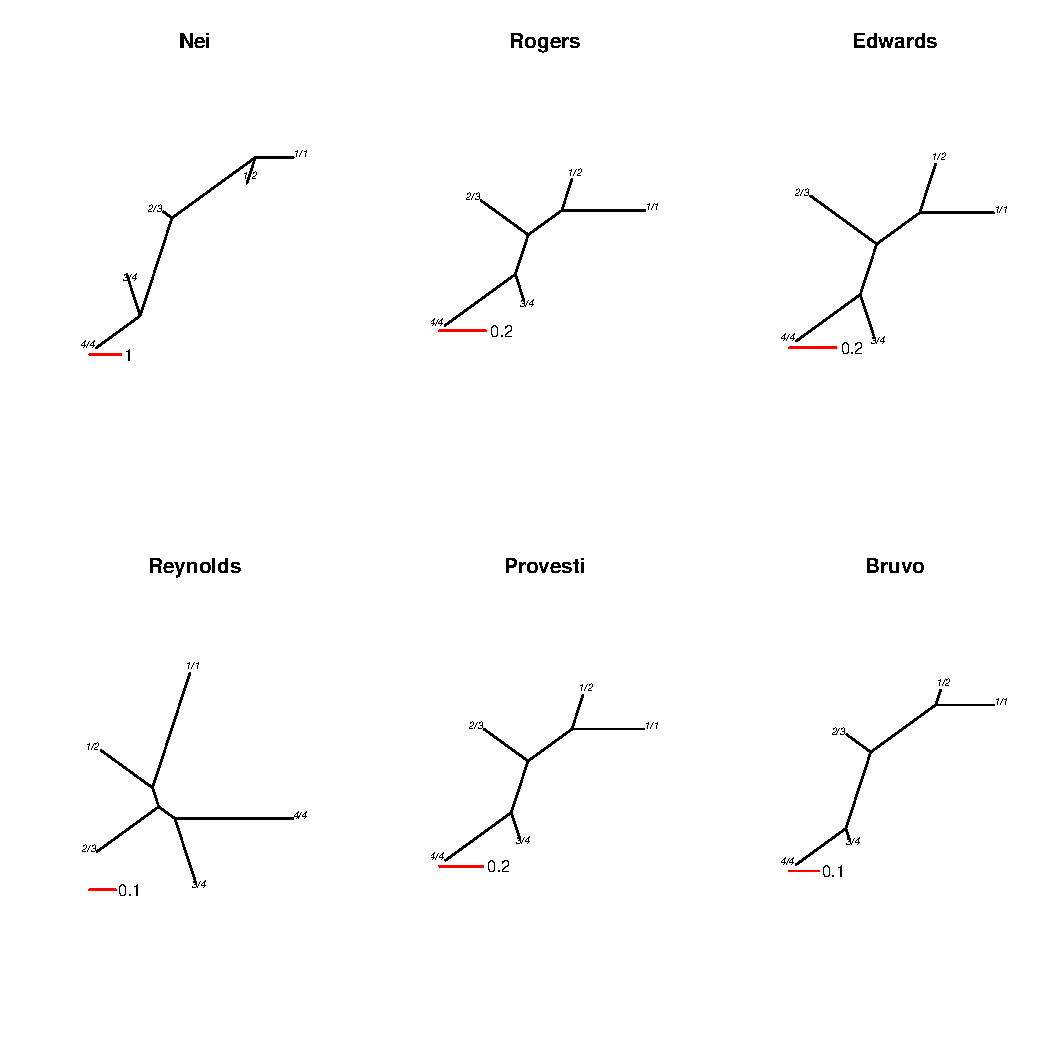
\includegraphics[width=0.95\linewidth]{figure/unnamed-chunk-3} 

}



\end{knitrout}

\section{AMOVA}

AMOVA in \poppr{} acts as a wrapper for the \textit{ade4} implementation, which
is an implementation of Excoffier's original formulation
\cite{excoffier1992analysis}. As the calculation relies on a genetic distance
matrix, \poppr{} calculates the distance matrix as the number of differing sites
between two genotypes using equation \ref{eq:ia_D}. This is equivalent to
Provesti's distance multiplied by the ploidy and number of loci. This is also
equivalent to Kronecker's delta as presented in \cite{excoffier1992analysis}. It
should also be mentioned that at this moment, it is not possible to calculate
AMOVA on polyploid data.

\section{Genotypic Diversity}

Many of the calculations of genotypic diversity exist within the package \textit{vegan} in the \texttt{diversity}
function. Descriptions of most of the calculations can be found in the paper by Gr\"unwald et al \cite{Grunwald:2003}.

\subsection{Rarefaction, Shannon - Wiener, Stoddart and Taylor indices}

Stoddart and Taylor's index is also known as Inverse Simpson's index.
A detailed description of these can be found in the ``Diversity'' vignette in \textit{vegan}. You can access it by typing \texttt{vignette("diversity-vegan")}

\subsection{Evenness ($E_{5}$)}
This is simply calculated as 

\begin{equation}
E_{5} = \frac{(1/\lambda) - 1}{e^{H}}
\end{equation}

Where $1/\lambda$ is Stoddart and Taylor's index and $H$ is Shannon diversity \cite{Stoddart:1988,Shannon:1948}.

\subsection{Hexp}

This one was cited as Nei's expected heterozygosity, but it has become clear
that it is not so. It was implemented in \poppr{} as it was in \textit{multilocus} \cite{Agapow:2001}. The calculation is as follows:

\begin{equation}
H_{exp} = \frac{N}{N-1} \sum_{i=1}^{g}{p^{2}_{i}}
\end{equation}
\noindent
Where $p_i$ is the frequency of the $i$th genotype, $g$ is the number of
genotypes observed and $N$ is the sample size. Essentially, it's an unbiased
estimator for the Simpson index.

\bibliographystyle{pnas.bst}
\bibliography{poppr_man}
\end{document}
